\documentclass[12pt]{article}
\usepackage[utf8]{inputenc}
\usepackage[T1]{fontenc}
\usepackage{amsmath}
\usepackage{amsfonts}
\usepackage{amssymb}
\usepackage[version=4]{mhchem}
\usepackage{stmaryrd}
\usepackage{hyperref}
\usepackage{graphicx}
\graphicspath{{../data/}}
\hypersetup{colorlinks=true, linkcolor=blue, filecolor=magenta, urlcolor=cyan,}
\urlstyle{same}


\usepackage{listings} % Required for insertion of code
\usepackage{xcolor} % Required for custom colors

% Define custom colors
\definecolor{codegreen}{rgb}{0,0.6,0}
\definecolor{codegray}{rgb}{0.5,0.5,0.5}
\definecolor{codepurple}{rgb}{0.58,0,0.82}
\definecolor{backcolour}{rgb}{0.95,0.95,0.92}

% Setup the style for code listings
\lstdefinestyle{mystyle}{
    backgroundcolor=\color{backcolour},   
    commentstyle=\color{codegreen},
    keywordstyle=\color{magenta},
    numberstyle=\tiny\color{codegray},
    stringstyle=\color{codepurple},
    basicstyle=\ttfamily\footnotesize,
    breakatwhitespace=false,         
    breaklines=true,                 
    captionpos=b,                    
    keepspaces=true,                 
    numbers=left,                    
    numbersep=5pt,                  
    showspaces=false,                
    showstringspaces=false,
    showtabs=false,                  
    tabsize=2
}

% Activate the style
\lstset{style=mystyle}

\title{Homework 1}
\author{Patryk Kozlowski} 

\begin{document}
\maketitle
\section{Problem 1}
This problem will familiarize you with the formulas commonly used in a nonlinear optics lab for computing powers, as well as try to give a relative scale to those powers. I encourage you to download the "APE Calculator" application so that you will always have a quick way of doing these calculations.

The following formulas are useful

Average Power, $P$, common units $(\mathrm{W})$.

Intensity, $I=\frac{P}{\text { area }}=\frac{c n \epsilon_{0}}{2}|E|^{2}$, common units $\left(\mathrm{W} / \mathrm{cm}^{2}\right)$

Energy of pulse, Energy $=P /\left(f_{\text {repetitionrate }}\right)$, common units $\mathrm{J}$

Peak Power or Intensity, $I_{\text {peak }}$ or $P_{\text {peak }}=\frac{(\text { IorP }) / f_{\text {repititionrate }}}{\tau_{\text {pulse }}}$, common units W

Calculate the peak power $(\mathrm{W})$, peak electric field $(\mathrm{V} / \mathrm{cm})$, and peak magnetic field (Tesla) for the following cases. Assume a Ti:Sapphire amplifier operating at a $1 \mathrm{kHz}$ repetition rate. Assume $\mathrm{n}=1$.

\subsection{}
An average excitation power for pump probe experiments is $10 \mathrm{~mW}$ into a $200 \mathrm{um}$ spot with a pulsed width of $50 \mathrm{fs}$.
\subsubsection{Answer}
This gives us the a peak power of $6.37 \times 10^{15} \mathrm{W}$, peak electric field of $3.07 \times 10^{7} \mathrm{V} / \mathrm{cm}$, and peak magnetic field of $1.02 \times 10^{-4} \mathrm{T}$.
% Inline Python code in the document

\subsection{}
An average power for a high harmonic experiment in which electrons are tunneled from a nucleus is $0.5 \mathrm{~W}$ into a $100 \mathrm{um}$ spot with a pulse width of $5 \mathrm{fs}$. (Note, the interatomic potential is $\sim 10^{9} \mathrm{~V} / \mathrm{m}$ by using the Coulomb potential and a separation of 0.5 Angstroms, hence tunneling can be achieved)
\subsubsection{Answer}
% can you round to the above sentence to 3 sig figs and also have at in the format that is redouble i.e. _.__ x 10{_}
The peak power is $1.27 \times 10^{19} \mathrm{W}$, peak electric field is $2.19 \times 10^{3} \mathrm{V} / \mathrm{cm}$, and peak magnetic field is $7.30 \times 10^{-4} \mathrm{T}$.

% Inline Python code in the document
% Inline Python code in the document
% Inline Python code in the document
\begin{lstlisting}[language=Python]
import math

# Constants
c = 3e8  # speed of light in m/s
epsilon_0 = 8.85e-12  # permittivity of free space in F/m
n = 1  # refractive index
f_repetition_rate = 1000  # Hz
tau_pulse = 5e-15  # pulse width in seconds
P = 0.5  # average power in Watts
diameter_um = 100
# get the  in cm
radius_m = diameter_um / 2e6

# Step 1: Area of the spot in m^2
area_m2 = math.pi * radius_m**2

I_avg = P / area_m2

P_peak = (I_avg / f_repetition_rate) / tau_pulse

# Step 5: Peak Electric Field in V/m
E_peak = math.sqrt(2 * I_avg / (c * n * epsilon_0))

# Convert E_peak to V/cm
E_peak_cm = E_peak / 100

# Step 6: Peak Magnetic Field in Tesla
B_peak = E_peak / c

P_peak, E_peak_cm, B_peak

\end{lstlisting}
\subsection{}
A high-field $\mathrm{THz}$ experiment would have an average power of $5 \mathrm{~mW}$ focused into $500 \mathrm{um}$ and a pulse width of $1 \mathrm{ps}$. (The DC dielectric breakdown field in most insulators is $10^{7} \mathrm{~V} / \mathrm{cm}$ )
\subsubsection{Answer}
This gives us the a peak power of $2.55 \times 10^{13} \mathrm{W}$, peak electric field of $43.8 \mathrm{V} / \mathrm{cm}$, and peak magnetic field of $1.46 \times 10^{-5} \mathrm{T}$.
% Inline Python code in the document
% Inline Python code in the document
\begin{lstlisting}[language=Python]
import math

# Constants
c = 3e8  # speed of light in m/s
epsilon_0 = 8.85e-12  # permittivity of free space in F/m
n = 1  # refractive index
f_repetition_rate = 1000  # Hz
tau_pulse = 1e-12  # pulse width in seconds
P = 0.005  # average power in Watts
diameter_um = 500
# get the  in cm
radius_m = diameter_um / 2e6

# Step 1: Area of the spot in m^2
area_m2 = math.pi * radius_m**2

I_avg = P / area_m2

P_peak = (I_avg / f_repetition_rate) / tau_pulse

# Step 5: Peak Electric Field in V/m
E_peak = math.sqrt(2 * I_avg / (c * n * epsilon_0))

# Convert E_peak to V/cm
E_peak_cm = E_peak / 100

# Step 6: Peak Magnetic Field in Tesla
B_peak = E_peak / c

P_peak, E_peak_cm, B_peak

\end{lstlisting}
\section{The Kramers-Kronig relationships:}
\subsection{}
Define the Kramers-Kronig relationships in plain words and how they work mathematically.
\subsubsection{Answer}
For physical quantities that we have discussed, like the susceptibility or dielectric, the Kramers-Kronig relationships provide a way to relate the real and imaginary parts of these physical quantities via integral transforms. Cauchy's residue theorem in complex analysis can be used to derive these. For example, the relationship for the dielectric function $\epsilon(\omega)$ is shown in Figure \ref{fig:kk}. The dielectric is decomposed into real and imaginary parts, as:
\begin{equation}
  \epsilon(\omega)=\epsilon_{1}(\omega)+i \epsilon_{2}(\omega)
\end{equation}
\begin{figure}
  \centering
  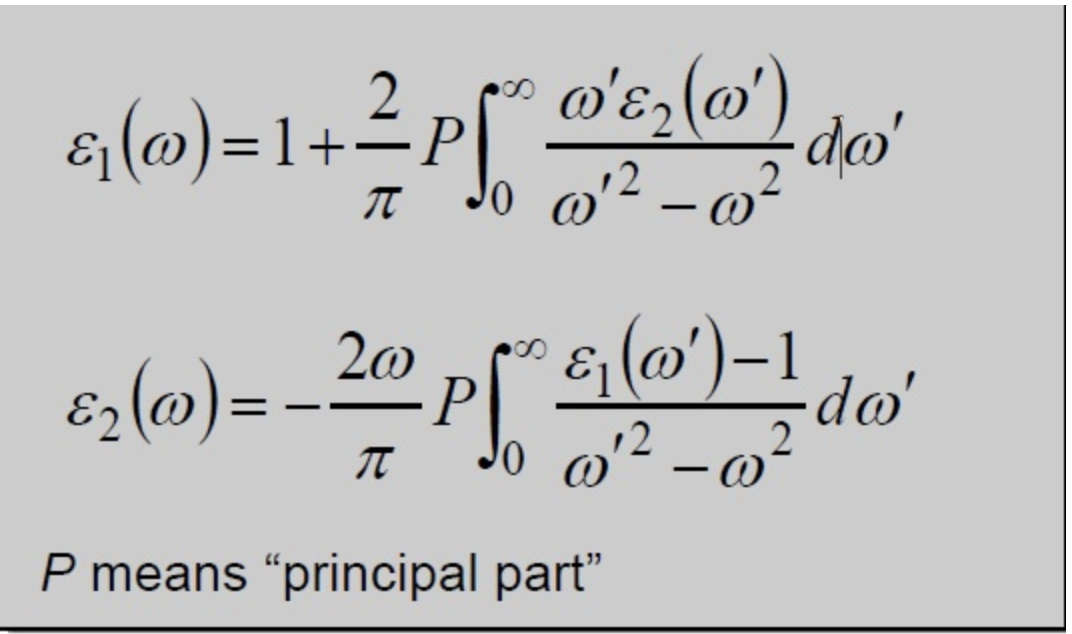
\includegraphics[width=\textwidth]{kk.png}
  \caption{Kramers-Kronig relationships for the dielectric function.}
  \label{fig:kk}
\end{figure}
\subsection{}
Why is it important to know the real or imaginary frequency components over a wide frequency range when doing a Kramers-Kronig transformation? What errors does it induce if not?
\subsubsection{Answer}
The situation with the Kramers-Kronig relationship can be thought of in analogy to the Fourier transform. If you knew of the value of a function very narrowly in frequency space, you would not be able to accurately determine the value of the function well in time space due to their relationship mediated by the integral transform. A similar concept applies to the Kramers-Kronig relationship; if you know the values of the real and imaginary parts of the dielectric function over a wide frequency range, you are fine, but if you only know one of them over a narrow range, this will induce errors in your computation of the other.
\subsection{}
For a Lorentzian oscillator, draw the real and imaginary parts of the dielectric function, and explain their curve shape in relation to the form of the Kramers-Kronig transformation.
\subsubsection{Answer}
\begin{figure}
  \centering
  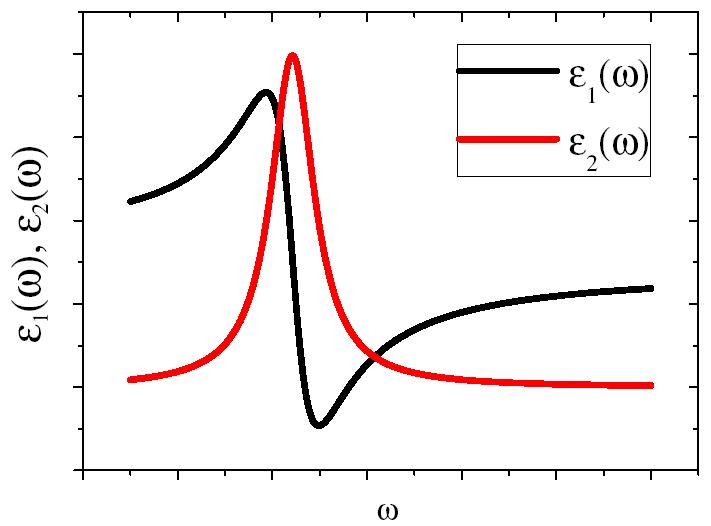
\includegraphics[width=\textwidth]{dielectric_plot.png}
  \caption{Real and imaginary parts of the dielectric function for a Lorentzian oscillator.}
  \label{fig:lorentzian}
\end{figure}
The real and imaginary parts of the dielectric function for a Lorentzian oscillator are shown in Figure \ref{fig:lorentzian}. The curved shape suggests that they are related by a derivative relationship which is what we would expect by looking at their relationship within the Kramers-Kronig transformation. We note that the real part is given by an odd function while the imaginary part is given by an even function.
\section{Problem 3}



 





This is another self-learning exercise since we do not have time in class to properly cover dispersion. Please go to \href{https://www.newport.com/n/the-effect-of-dispersion-on-ultrashort-pulses}{https://www.newport.com/n/the-effect-of-dispersion-on-ultrashort-pulses} . For this problem, draw the plot in Figure 2 and explain in words why this result exists. Note they use $20 \mathrm{~mm}$ of BK7, the average optic is closer to $2 \mathrm{~mm}$, but they add up quickly!
\subsection{}
\subsubsection{Answer}
In the figure \ref{fig:dispersion}, we see that when there is a very wide input pulse, the output pulse is equally wide. However, when the input pulse is very narrow, the output pulse widens. We observe this phenomenon because the wide pulse contains a narrow range of frequencies, so the dispersion affects each of these in a similar fashion. However, when the input pulse is narrow, the frequency spectrum is broad and so the dispersion affects each of these frequencies differently, leading to a broadening of the pulse. We call this phenomenon that leads to the broadening of the pulse group velocity dispersion.
\begin{figure}[h]
  \centering
  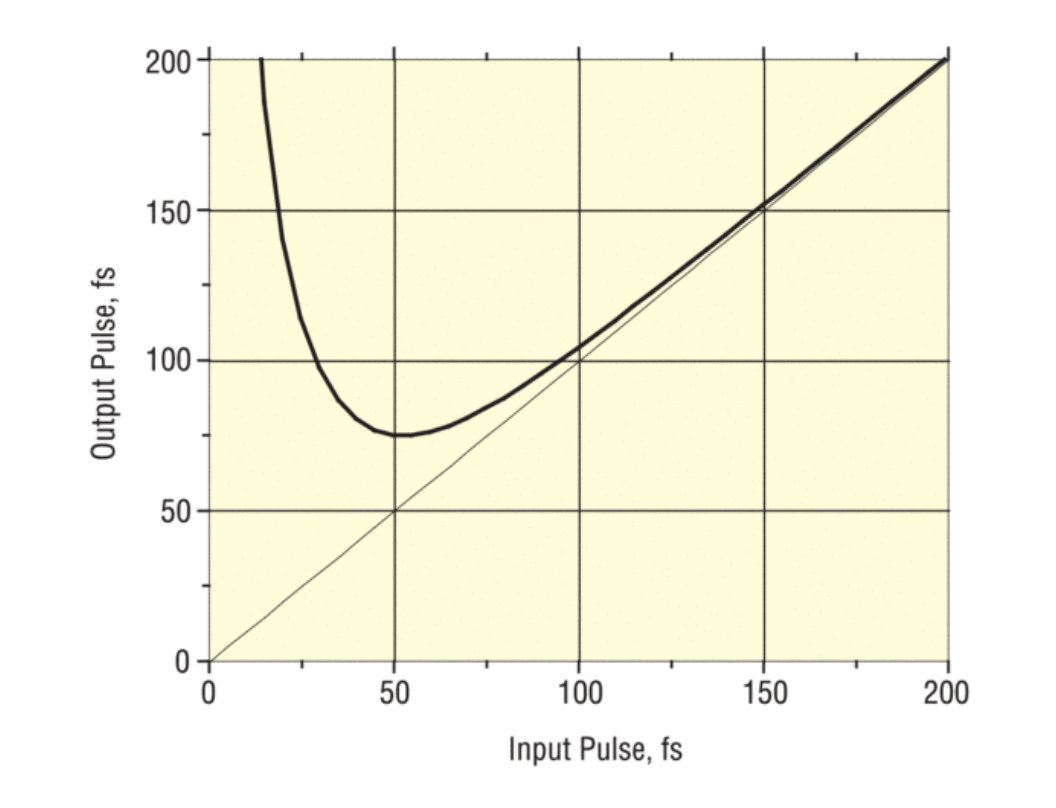
\includegraphics[width=\textwidth]{plot.png}
  \label{fig:dispersion}
\end{figure}
\end{document}